%!TEX program=xelatex
\documentclass{article}

\usepackage{ctex}
\usepackage{amsmath}
\usepackage{amssymb}
\usepackage{graphicx}
\usepackage{threeparttable}
\newcommand{\adots}{\mathinner{\mkern2mu%
\raisebox{0.1em}{.}\mkern2mu\raisebox{0.4em}{.}%
\mkern2mu\raisebox{0.7em}{.}\mkern1mu}}


\usepackage{url}

\title{第一次大作业} 
\author{陈文宇
	\and 徐维震
	\and 刘小端
	\and 高鹏智
	\and 阴雅萱} 
\date{\today}


\begin{document}
	\maketitle
	\begin{titlepage}
		\begin{abstract}
			学习latex使我快乐
		\end{abstract}
	\end{titlepage}

	
	\newpage
	\tableofcontents 	%自动生成目录
	\listoftables		%自动生成表格浮动体目录
	\listoffigures		%自动生成插图浮动体目录
	\newpage
	\section[教学测试]{教学测试\LaTeX}
	
	\subsection{不换行的公式编辑}
	a,b,c的关系为~\ $ a + b  = c $,(\(a + b = c\))\footnote{我瞎编的} %底部注释栏
	\begin{math} 
		a + b = c 
	\end{math}	
	\marginpar{\footnotesize 还是我瞎编的}
	
	\subsection{换行居中的公式编辑}
	
	a,b,c的关系如下:
	$$ a + b =c $$
	\marginpar{\footnotesize 依旧是我瞎编的} %侧栏注释栏
	
	
	且a,b,c满足:
	\[a * b = c\]
	
	\subsection{希腊字母}
	$\omega$,$\pi$,$\sigma$,$\alpha$,$\gamma$,$\beta$%可以在左侧结构栏快速寻找

	\subsection{上下标}
	$x^2 - 2x + 1 = 0 $,$y_2 - y_1=0$ % ^{}  _{}
	
	% $$公式$$可以换行居中
	\subsection{数学公式}
	
	$$ y=\sin^2 x+\cos^2 x $$ \label{eq:firsteq}
	$$ y=\log_3 x $$ 
	$$ y=\ln x $$ 
	$$ y=\sqrt[2]{x^2 +1} $$ 
	
	参见\ref{eq:firsteq}
	
	\subsection{分式}
	$1/3$ $$\frac{1}{3}$$ 
	$\frac{x^2+1}{x^3-1}$
	\begin{math}
		\frac{x^3+1}{x^4+2}
	\end{math}\\

	\subsection{行间公式}
	$$\frac{x^2+1}{x^3-1}$$
	\[\frac{x^2+1}{x^3-1}\]
	\begin{displaymath}
		\frac{x^2+1}{x^3-1}
	\end{displaymath}
	
	\subsection{自动编号的equation环境(可引用)}
	交换律详见公式(\ref{eq:com1}),结合律详见公式(\ref{eq:com2})
	\begin{equation}
		a+b=b+a\label{eq:com1}
	\end{equation}
	\begin{equation}
	(a*b)*c=a*(b*c)\label{eq:com2}
	\end{equation}
	\begin{equation*}
	(a*b)*c=a*(b*c)
	\end{equation*}
		%其中可以使用equation*来设置不编号的等式,
		%但是equation*需要引用宏包amsmath
	
	\section{特殊环境}
	
	\subsection{列表}
	\begin{center}
	\begin{tabular}{| @{~: } |r| @{~: } |l| |r|@{}|}
	\hline \hline
	1 & 1 & one\\
	11& 3 & eleven\\
	\hline
	\end{tabular}
	\end{center}
	
	\subsection{插图}
	\begin{center}	
		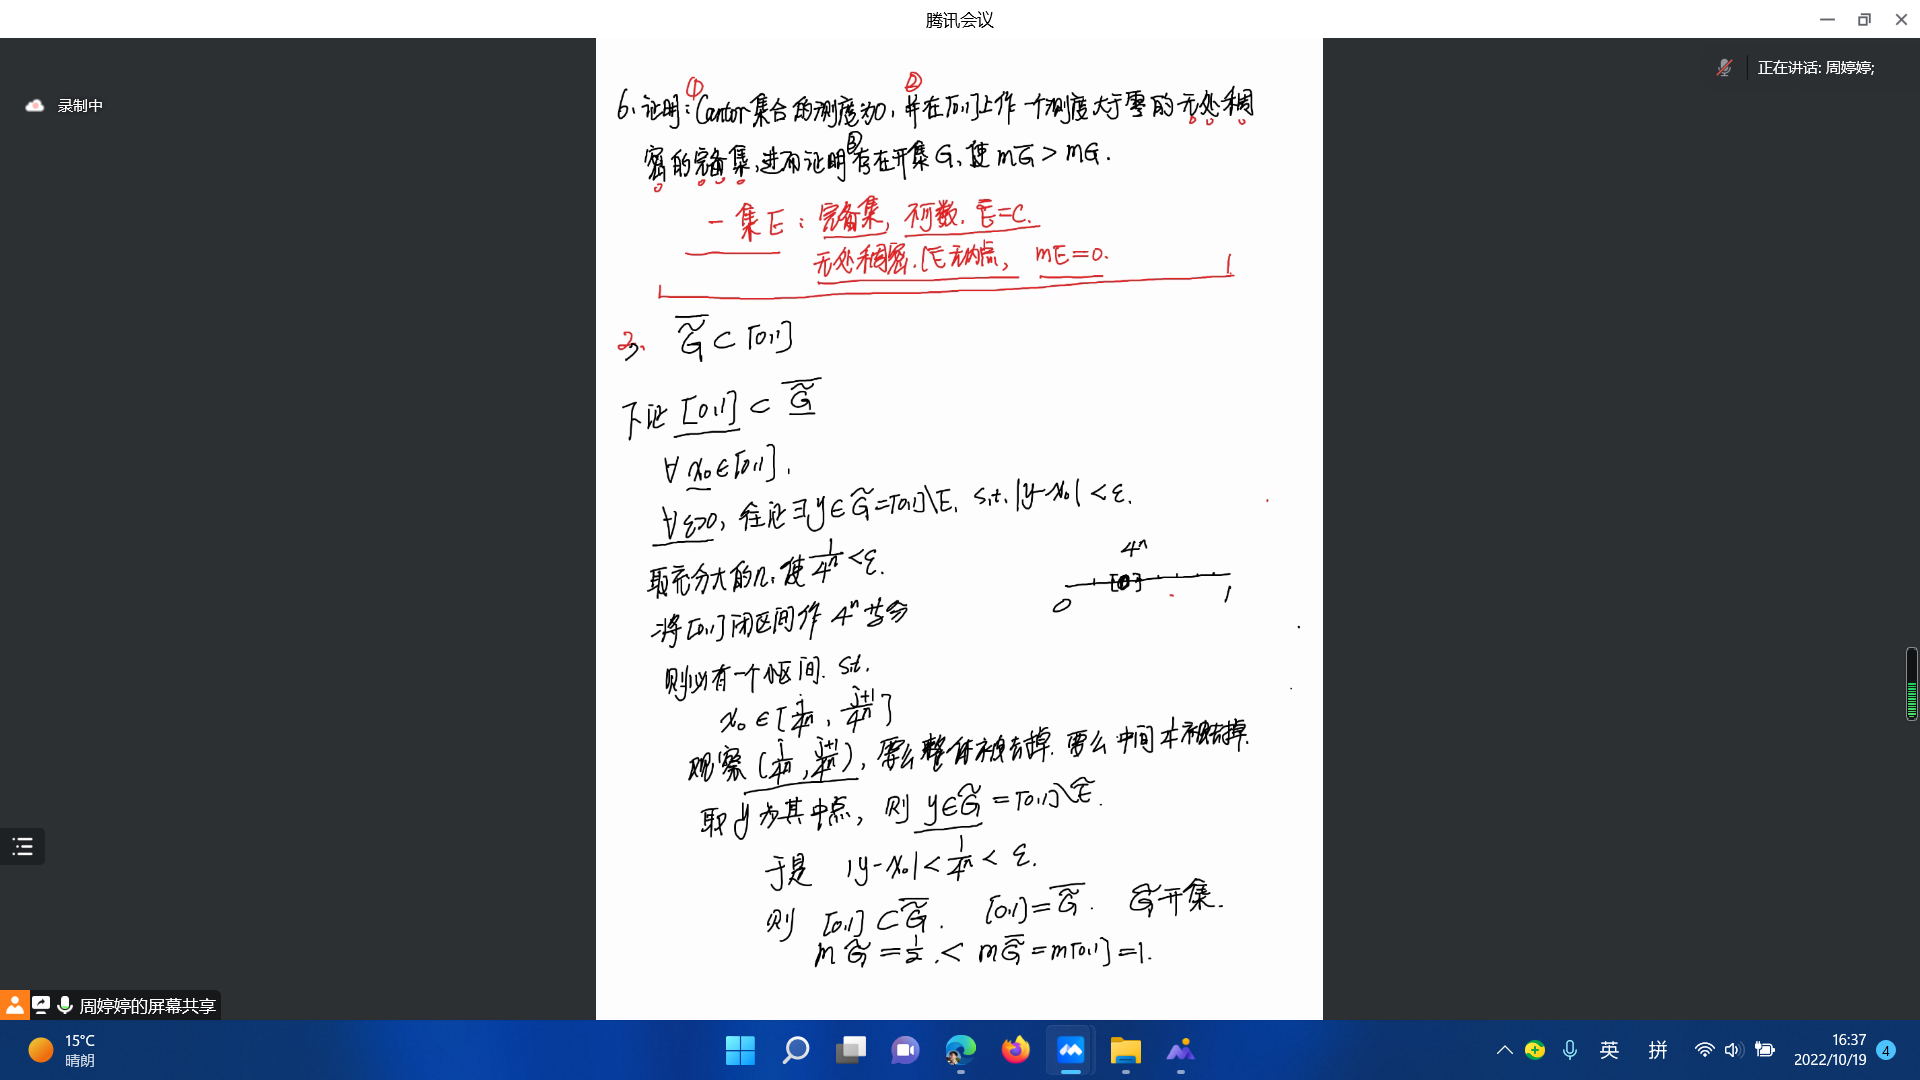
\includegraphics[scale=0.2]{屏幕截图(196)}%需要宏包\graphicx
	\end{center}
	

	\subsection{盒子}
	%基本的盒子
	|\mbox{\\mbox命令可以生成一个最基本的盒子}| \\
	%宽度为25em
	|\makebox[25em]{\\makebox命令可以生成一个最基本的盒子}| \\		%默认居中对齐
	|\makebox[25em][l]{\\makebox[][l]命令可生成一个最基本的盒子}| \\	 %左对齐
	|\makebox[25em][r]{\\makebox[][r]命令能生成一个最基本的盒子}| \\	 %右对齐
	|\makebox[25em][s]{\\makebox[][s]命令 会生成一个 最基本的盒子}|   %分散对齐
	
	%有边框的盒子
	|\fbox{\\mbox命令可以生成一个最基本的盒子}| \\
	%宽度为25em
	|\framebox[25em]{\\framebox命令可以生成一个最基本的盒子}| \\		%默认居中对齐
	|\framebox[25em][l]{\\framebox[][l]命令可生成一个最基本的盒子}| \\	 %左对齐
	|\framebox[25em][r]{\\framebox[][r]命令能生成一个最基本的盒子}| \\	 %右对齐
	|\framebox[25em][s]{\\framebox[][s]命令 会生成一个 最基本的盒子}|   %分散对齐
	
	%垂直盒子
	三字经:\parbox[t]{3em}%
	{人之初 性本善 性相近 习相远}
	\qquad
	千字文:
	\begin{minipage}[b][8ex][t]{4em}
		天地玄黄 宇宙洪荒
	\end{minipage}

	%迷你页
	\fbox{\begin{minipage}{15em}%
			这是一个垂直盒子的领域。
			\footnote{脚注来自迷你业}
	\end{minipage}}
	
	%标尺盒子
	\rule{12pt}{4pt},\rule[4pt]{6pt}{8pt},\rule[-4pt]{6pt}{8pt},\rule[-.4pt]{3em}{.4pt}
	
	
	
	\subsection{浮动体}
	浮动体位置参数的设定参见表\ref{表1}
	\begin{table}[h]
		\caption{浮动体的位置参数}\label{表1}
		\centering
		\begin{threeparttable}
			\begin{tabular}{ll}
				\hline
				参数 & 含义\\
				\hline
				h   &  当前位置(代码所处的上下文)\\
				t   &  顶部\\
				b   &  底部\\
				p   &  单独成页\\
				!   &  在决定位置是忽视限制\\
				\hline
			\end{tabular}
		\end{threeparttable}
	
		\begin{tablenotes}
			
			\footnotesize
			\item 注1:这是浮动体的位置参数
		\end{tablenotes}
		
	\end{table}

	\begin{figure}[htbp]
		\centering
		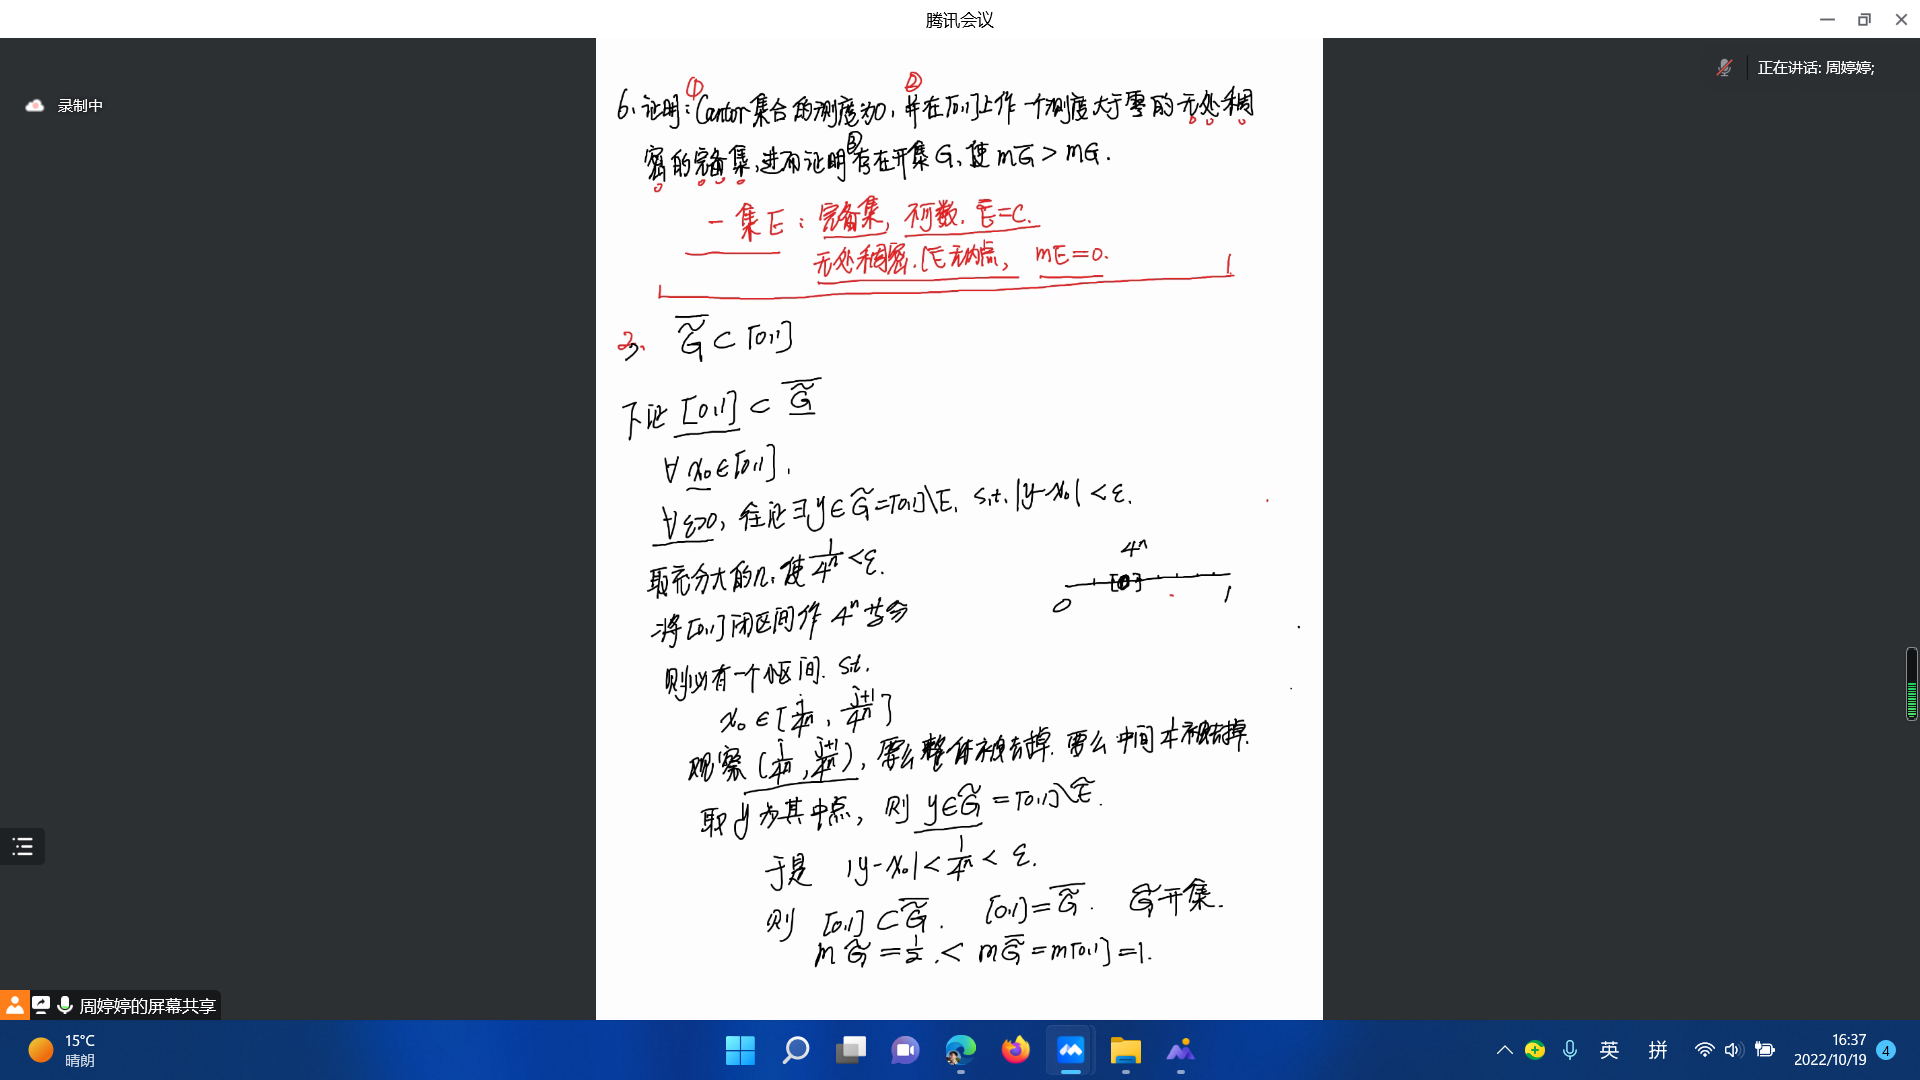
\includegraphics[scale=0.08]{屏幕截图(196)}
		\qquad
		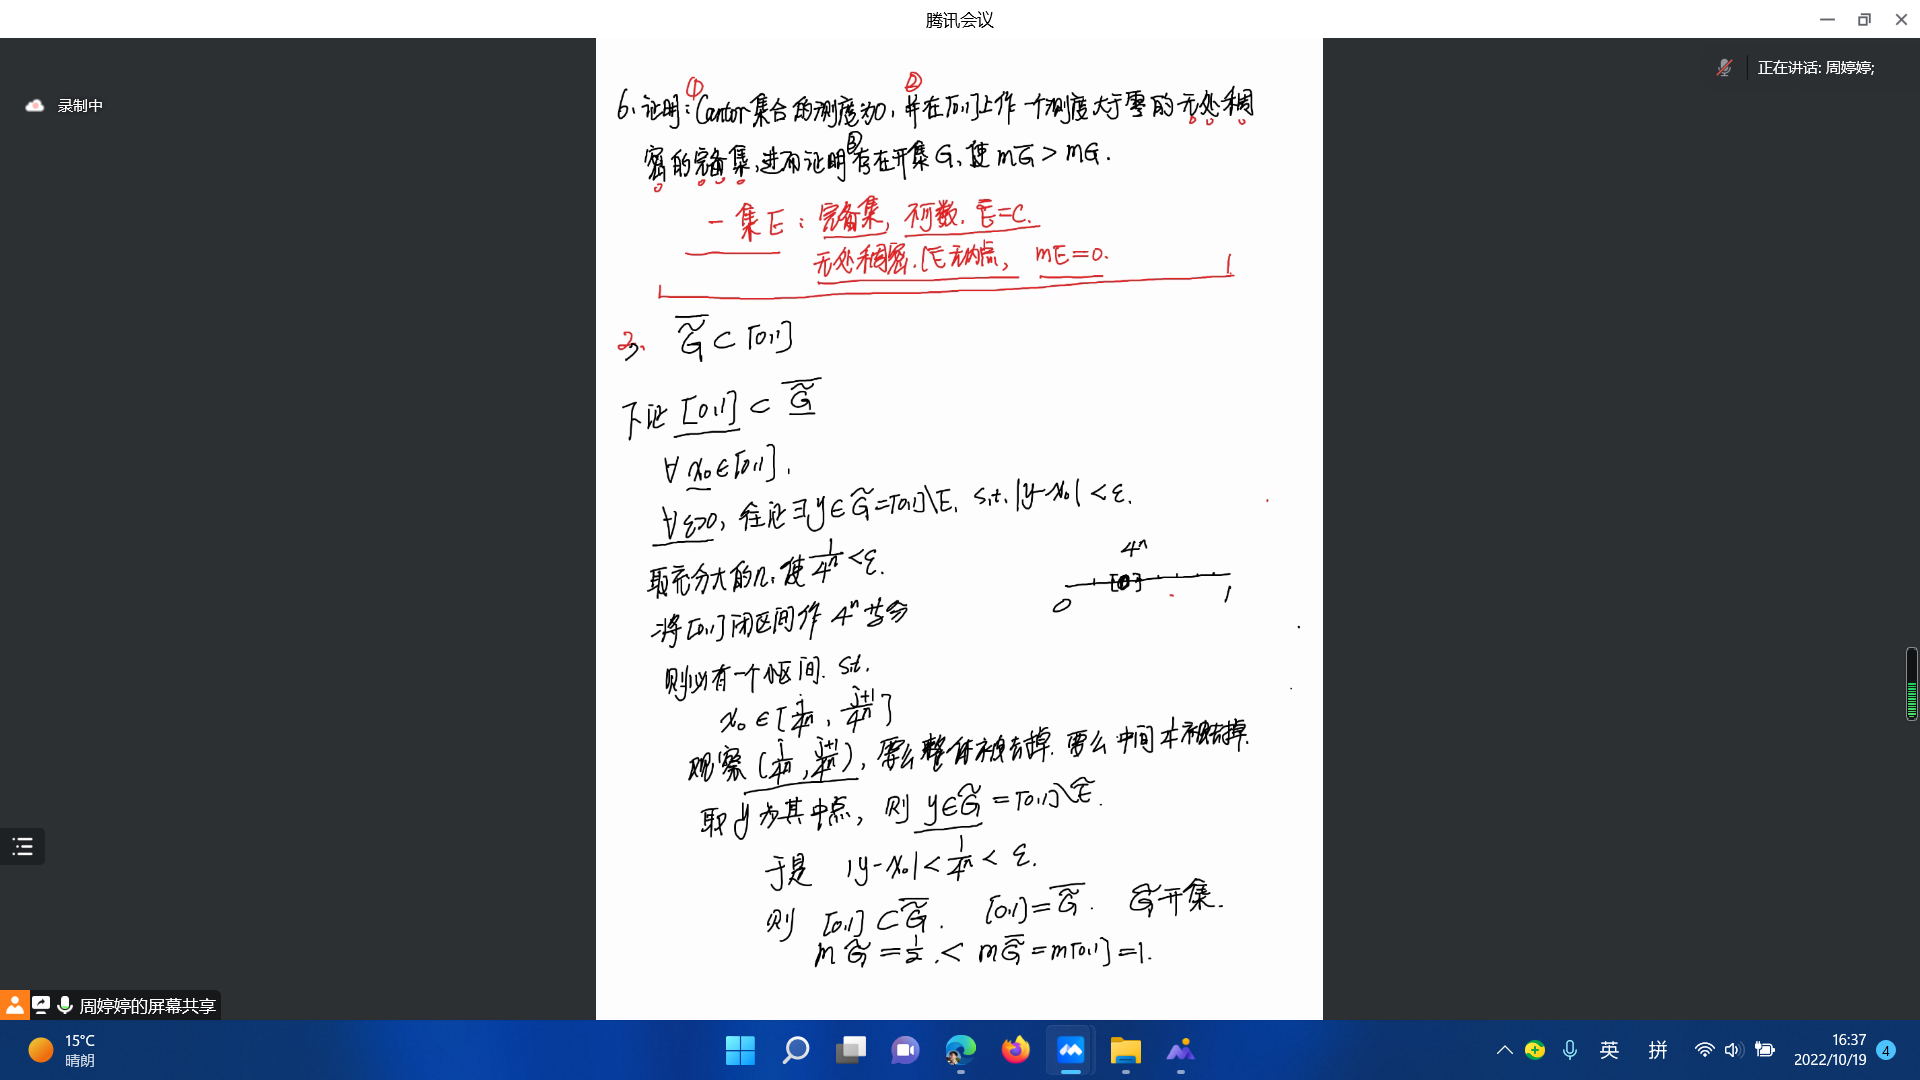
\includegraphics[scale=0.08]{屏幕截图(196)}
		\\[10pt]
		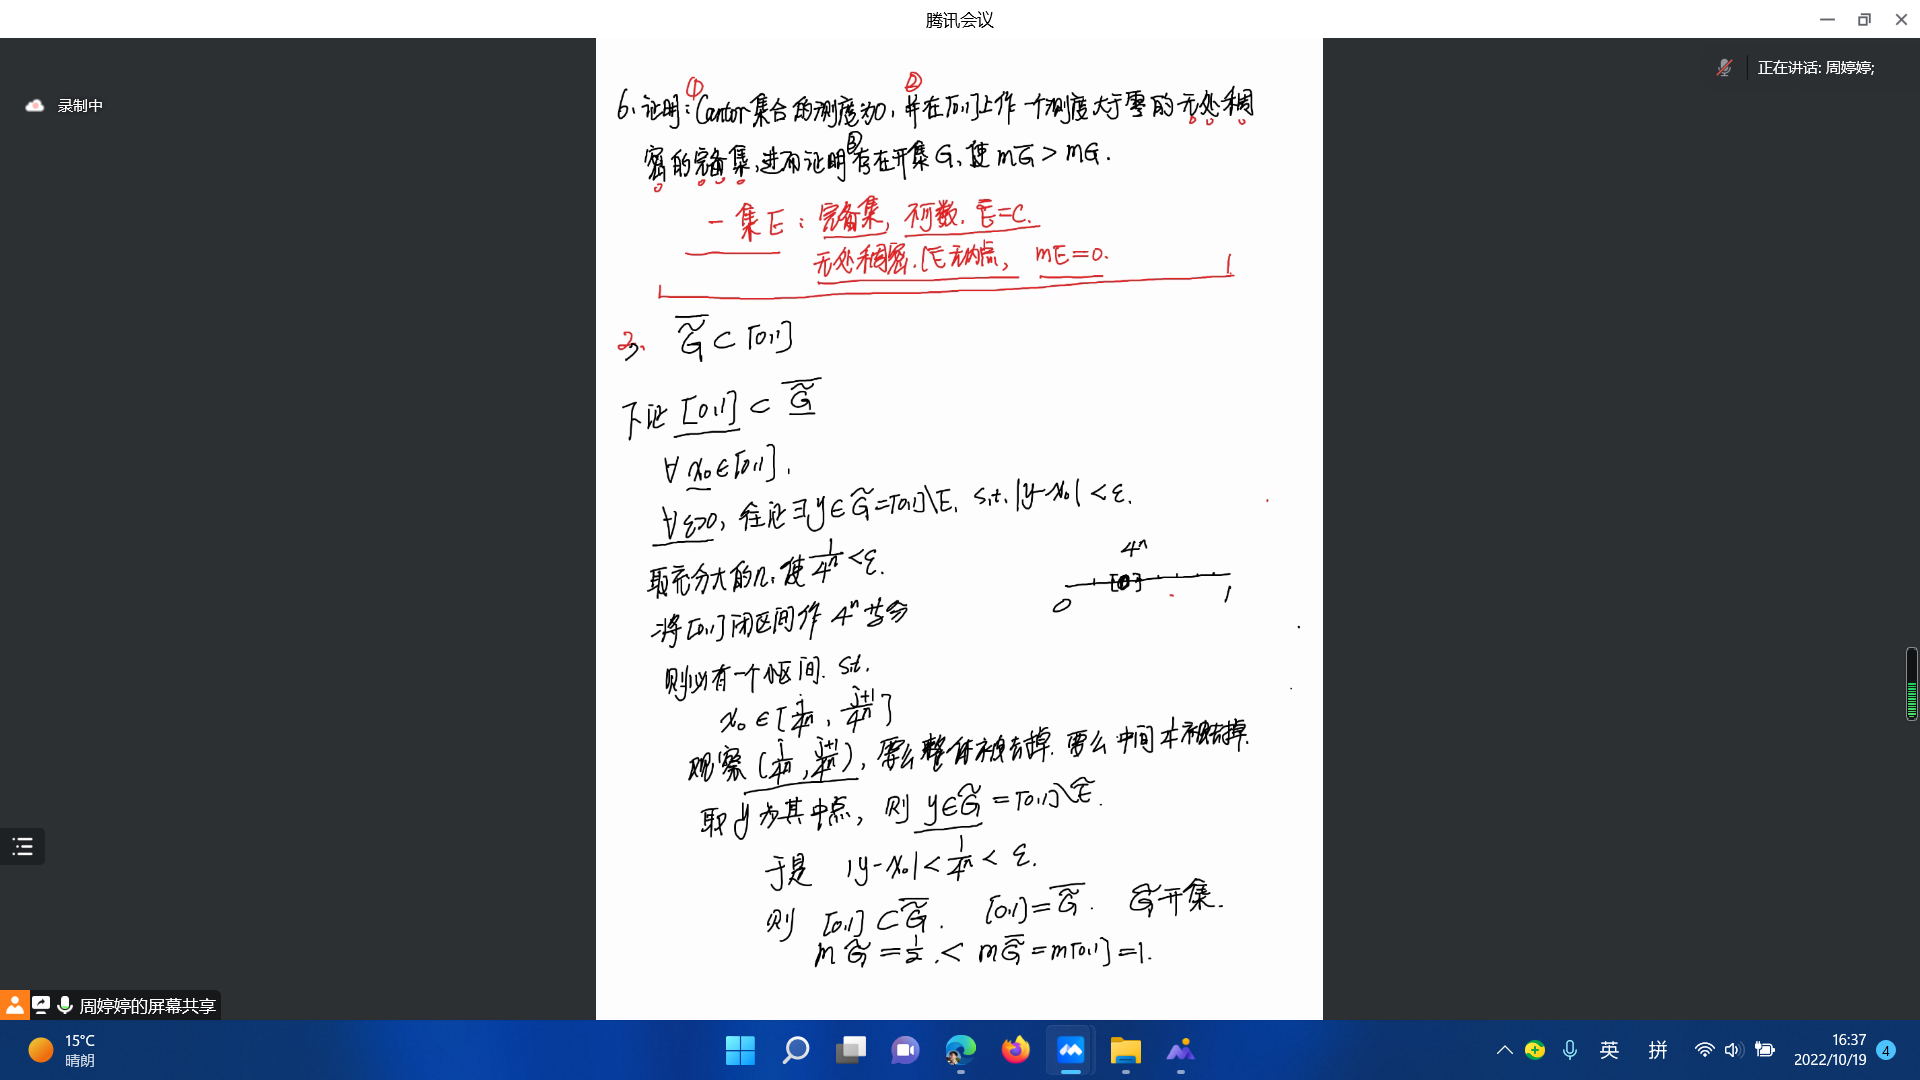
\includegraphics[scale=0.17]{屏幕截图(196)}
		\caption{随便的插图}
	\end{figure}
	

	
	%用\
	\subsection{gather环境和gather*环境}
	%gather环境可以给出大量的公式并编号
	%gather*环境不可以,事实上 环境名* 就是代表该环境不\label{key}的意思
	\begin{gather}
		a \times b = c\\
		b \times a = c
	\end{gather}
	\begin{gather*}
		a \times b = c\\
		b \times a = c
	\end{gather*}


	
	\section[数学矩阵的基本形式]{数学矩阵的基本形式}
	\(
	\begin{matrix}
		1 & 0 \\
		0 & 1 
	\end{matrix}
	\) \qquad
	\(
	\begin{pmatrix}
		1 & 0 \\
		0 & 1 
	\end{pmatrix}
	\) \qquad
	\(
	\begin{bmatrix}
		1 & 0 \\
		0 & 1 
	\end{bmatrix}
	\) \qquad
	\(
	\begin{Bmatrix}
		1 & 0 \\
		0 & 1 
	\end{Bmatrix}
	\) \qquad
	\(
	\begin{vmatrix}
		1 & 0 \\
		0 & 1 
	\end{vmatrix}
	\) \qquad
	\(
	\begin{Vmatrix}
		1 & 0 \\
		0 & 1 
	\end{Vmatrix}
	\) \\
	\[
	A=
	\begin{bmatrix}
		1 & 0 \\
		0 & 1 
	\end{bmatrix}
	\]
	
	\subsection{数字矩阵的常用省略符} %\dots、\vdots、\ddots、\adots(需要自己定义)
	\[
	A=
	\begin{bmatrix}
		a_{11} & \dots & a_{1n} \\
		       & \ddots& \vdots \\
		0      &       & a_{nn}
	\end{bmatrix}
	\]	
	
	\[
	A=
	\begin{bmatrix}
			0  & \dots  & a_{1n}  \\
		 \vdots& \adots & \vdots  \\
		a_{n1} & \dots  & a_{nn}
	\end{bmatrix}
	\]
	\subsection{分块矩阵}
	\[
	%分块矩阵的编写
	\begin{bmatrix}

	\begin{matrix}	1 & 0 \\ 0 & 1 \end{matrix} 
	& \text{\large 0} \\
	\text{\large 0}  
	& \begin{matrix} 0 & -1 \\ 1 & 0\end{matrix}
	
    \end{bmatrix}
	\]
	
	\subsection{三角矩阵}
	\[
	\begin{bmatrix}
		a_{11} & a_{12} & \dots & a_{1n} \\
		       & a_{22} & \dots & a_{2n} \\
		       &   		& \ddots& \vdots \\
		\multicolumn{2}{c}{\raisebox{1.3 ex}[0 pt]{\huge 0}} &       & a_{nn} 
	\end{bmatrix}
	\]
	
	\subsection{跨列的省略号}%\hdotsfor{columns}
	\[
	\begin{bmatrix}
		1&2&3&4\\
		\hdotsfor{4}\\
		9&10&11&12
	\end{bmatrix}
	\]
	
	\subsection{行内小矩阵}
	复数 $z=(x,y)$ 还可以用矩阵
	\begin{math}
		\left(%需要手动添加左括号
		\begin{smallmatrix}
			x&-y\\y&x
		\end{smallmatrix}
		\right)%需要手动添加右括号
	\end{math}
	来表示
	
	\subsection{array环境}
	\[
	\begin{array}{c|c}
		\frac{1}{2} & 0 \\
		\hline
		0 & \frac{a}{b}
	\end{array}
	\]
	
	%用array构造复杂矩阵
	%@{<内容>}--表示添加任意内容,不占表项计数
	%吃=此处添加一个负值空白,表示左移5pt的距离
	\[
	\begin{array}{c@{\hspace{-5pt}}l}
		%第一行第一列
		\left(
		\begin{array}{ccc|ccc}
			a & \dots  & a     & b    & \dots & b \\
			  & \ddots & \vdots&\vdots& \adots&   \\
			  &        & a     & b    &       &   \\
			\hline
			  &        &       & c    & \dots & c \\
			  &        &       &\vdots&       &\vdots \\
		  \multicolumn{3}{c|}{\raisebox{2ex}[0pt]{\Huge 0}}
		  &c &\dots &c		  
		\end{array}
		\right)
		&
		\begin{array}{l}
			\left.\rule{0mm}{9mm}\right\}p \\
			\left.\rule{0mm}{9mm}\right\}q
		\end{array}\\[-5pt]
		\begin{array}{cc}
			\underbrace{\rule{17mm}{0mm}}_m&
			\underbrace{\rule{17mm}{0mm}}
		\end{array}
		&	
	\end{array}
	\]


	日本人口老龄化影响\cite{2020}
	
	“数值分析”课程教学探讨\cite{2021}
	
	基于LaTeX的Web数学\cite{2022}
	
	\section[参考文献的编辑]{参考文献的编辑}
	%\begin{thebibliography}{99}
	%	\bibitem{acticle1}陈立辉,苏伟,蔡川,陈晓薇.\emph{基于LaTeX的Web数学%公式提取方法的研究}[J]. 计算机科学.2014(06)
	%\end{thebibliography}

%	\nocite{*}
%	这是一个引用文件\cite{noauthor__nodate}

	\bibliographystyle{plain}
	\bibliography{cnki}
	%\nocite{*}
		
		
	


	
	
	\section{代码展示}
	\begin{verbatim}
		#include<stdio.h>
		#include<stdlib.h>
		#include<math.h>
		
		//1.编写 h1 函数 
		//2.编写 h2 函数 
		//3.带入结点,每个函数都会返回一个函数值,将其相乘,
		//	 4个这样的乘积加权后得到每部分的函数值
		//4.三个部分函数值相加为插值多项式的值 p
		//主函数:定义参数,初始化,调用 p 即可 
		
		//编写 h1 h2 利用其 封装在 p 函数里 
		double h1(int T,int j,double x[],double xs);
		double h2(int T,int j,double x[],double xs);
		double px1(double xs,double ys,int N,int m
		    ,double x[],int n,double y[],double f[],double fx[],double fy[],double fxy[]);
		double px2_ex(double xs,double ys,int N,int m,
		    ,double x[],int n,double y[],double f[],double fx[],double fy[]);
		double px2(double xs,double ys,int N,int m,double x[],int n,double y[],
		    ,double f[],double fx[],double fy[]); 
		double l_2(int T,int j,double x[],double xs);
		
		int main(){
			//给出 结点指标 N*N 
			//待求点(xs,ys)所在分片位置(x[m],y[n]),(x[m+1],y[n]),(x[m],y[n+1]),(x[m+1],y[n+1])
			//步长h,结点(x[],y[]) 
			//录入 f fx fy fxy 的值 
			// 返回 待求点的插值多项式的值 p 
			int N=6,m,n,i,j;
			double h;
			double x[N],y[N];
			double f[N*N],fx[N*N],fy[N*N],fxy[N*N];
			double xs=1.0/3.0,ys=2.0/3.0;
			double p;
			
			//初始化
			h=1.0/(N-1);
			for(i=0;i<N;i++){
				x[i]=h*i;
				y[i]=h*i;
			}
			for(i=0;i<N;i++){
				for(j=0;j<N;j++){
					f[j*N+i]=sin(pow(x[i],2)*y[j]+1);
					fx[j*N+i]=2*x[i]*y[j]*cos(pow(x[i],2)*y[j]+1);
					fy[j*N+i]=pow(x[i],2)*cos(pow(x[i],2)*y[j]+1);
					fxy[j*N+i]=2*x[i]*cos(pow(x[i],2)*y[j]+1)
						-2*pow(x[i],3)*y[j]*sin(pow(x[i],2)*y[j]+1);
				}		
			}
			/*
			int M=10;
			h=0.2/M;
			for(i=1;i<M;i++){
				
				xs=0.2+h*i;
				m=floor((N-1)*xs);
				
				ys=0.4+1e-6;
				n=floor((N-1)*ys);
				p=px2(xs,ys,N,m,x,n,y,f,fx,fy);
				printf("question2:待求点插值多项式的为:%.12lf\n",p);
				
				ys=0.4-1e-6;
				n=floor((N-1)*ys);
				p=px2(xs,ys,N,m,x,n,y,f,fx,fy);
				printf("question2:待求点插值多项式的为:%.12lf\n",p);
				
				printf("\n");		
				
			}
			*/
			
			m=floor((N-1)*xs);
			
			n=floor((N-1)*ys);
			
			p=px1(xs,ys,N,m,x,n,y,f,fx,fy,fxy);
			
			printf("question1:待求点插值多项式的为:%.12lf\n",p);
			
			p=px2_ex(xs,ys,N,m,x,n,y,f,fx,fy);
			
			printf("question2:基于算法一的待求点插值多项式的值为:%.12lf\n",p);	
			
			p=px2(xs,ys,N,m,x,n,y,f,fx,fy);
			
			printf("question2:基于算法二的待求点插值多项式的为:%.12lf\n",p);
			
		} 
		
		double h1(int T,int j,double x[],double xs){
			double h;
			if(T==0){
				h=pow((xs-x[j+1])/(x[j]-x[j+1]),2)*(1-2*(xs-x[j])/(x[j]-x[j+1]));
			}
			if(T==1){
				h=pow((xs-x[j])/(x[j+1]-x[j]),2)*(1-2*(xs-x[j+1])/(x[j+1]-x[j]));
			}
			
			return h;
		}
		
		double h2(int T,int j,double x[],double xs){
			double h;
			if(T==0){
				h=pow(((xs-x[j+1])/(x[j]-x[j+1])),2)*(xs-x[j]);
			}
			if(T==1){
				h=pow(((xs-x[j])/(x[j+1]-x[j])),2)*(xs-x[j+1]);
			}
			
			return h;
		}
		
		double l_2(int T,int j,double x[],double xs){
			double h;
			if(T==0){
				h=pow(((xs-x[j+1])/(x[j]-x[j+1])),2);
			}
			if(T==1){
				h=pow(((xs-x[j])/(x[j+1]-x[j])),2);
			}
			
			return h;
		}
		
		double px1(double xs,double ys,int N,int m,
			,double x[],int n,double y[],double f[],double fx[],double fy[],double fxy[]){
			double p=0;
			int i,j;
			
			for(i=0;i<=1;i++){
				for(j=0;j<=1;j++){
					p+=h1(i,m,x,xs)*h1(j,n,y,ys)*f[(n+j)*N+m+i]		//给出part1的值
					+h2(i,m,x,xs)*h1(j,n,y,ys)*fx[(n+j)*N+m+i]	//给出part2的值 
					+h1(i,m,x,xs)*h2(j,n,y,ys)*fy[(n+j)*N+m+i] 
					+h2(i,m,x,xs)*h2(j,n,y,ys)*fxy[(n+j)*N+m+i];//给出part3的值
				}
			}
			
			return p;
		}
		
		double px2_ex(double xs,double ys,int N,int m
			,double x[],int n,double y[],double f[],double fx[],double fy[]){
			double p=0;
			int i,j;
			
			for(i=0;i<=1;i++){
				for(j=0;j<=1;j++){
					p+=h1(i,m,x,xs)*h1(j,n,y,ys)*f[(n+j)*N+m+i]		//给出part1的值
					+h2(i,m,x,xs)*h1(j,n,y,ys)*fx[(n+j)*N+m+i]	//给出part2的值 
					+h1(i,m,x,xs)*h2(j,n,y,ys)*fy[(n+j)*N+m+i];
					
				}
			}
			
			return p;
		}
		
		
		double px2(double xs,double ys,int N,int m,double x[],int n
			,double y[],double f[],double fx[],double fy[]){
			double p1=0,p2=0,p;
			int i,j;
			
			//给出part1的值 
			for(i=0;i<=1;i++){
				for(j=0;j<=1;j++){
					p1=p1+(h1(i,m,x,xs)*l_2(j,n,y,ys)+h1(j,n,y,ys)*l_2(i,m,x,xs)
							-l_2(i,m,x,xs)*l_2(j,n,y,ys))*f[(n+j)*N+m+i];
				}
			}
			//给出part2的值 
			for(i=0;i<=1;i++){
				for(j=0;j<=1;j++){
					p2=p2+h2(i,m,x,xs)*l_2(j,n,y,ys)*fx[(n+j)*N+m+i]
						+l_2(i,m,x,xs)*h2(j,n,y,ys)*fy[(n+j)*N+m+i];
				}
			}
			
			p=p1+p2;
			
			return p;
			
		}
		
	\end{verbatim}
	
\end{document}